\chapter{Ứng dụng triển khai}
Nói về ứng dụng xây dựng sử dụng rails
\section{View trong Rails}
View là thành phần dùng để hiển thị dữ liệu từ model được cung cấp bởi controller, view là thành phần mà các triết lý của Rails được thể hiện rõ nhất, bằng việc hỗ trợ tự động sinh mã sử dụng method render.
Mỗi view được biểu diễn bởi một file có phần mở rộng .html.erb và tương ứng với một method trong controller tương ứng, tất cả các view của một controller được đặt trong một thư mục có tên là controller đó nằm trong thư mục app/view, hình ~\ref{fig:d} là cấu trúc của một project Rails chuẩn.
\begin{figure}
	\centering
		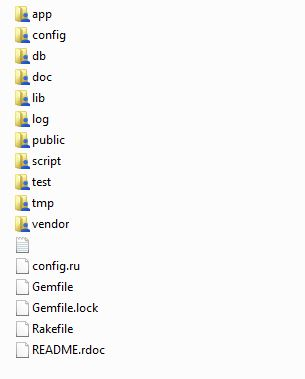
\includegraphics{image/d.JPG}
	\caption{Cấu trúc 1 project Rails}
	\label{fig:d}
\end{figure}
